\section{Design Decisions and Rationale}

The visual and interactive design of the \textit{Dota Stats} web application has been designed to meet the needs of its target users -- Dota 2 players, enthusiasts, and content creators, while prioritizing clarity and performance. This section explains the main design choices made for layout, interaction patterns, color schemes, and typography, along with the rationale behind each decision.

\subsection{Layout}

A dashboard-style layout with clearly separated sections for Player Profile, Hero Stats, Heroes Meta, and Selected Hero Page.
\\
\\
This layout supports the analytical nature of the application, allowing users to quickly locate complex data. Casual and competitive players benefit from structured content areas where different data types (e.g. win rates, hero performance, match history) are logically grouped, minimizing cognitive load, and reducing navigation effort.

\subsection{Interaction Patterns}

Search-based interaction for profile lookup, sortable tables for stats, and tab-based navigation.
\\
\\
Users interact primarily by entering their player ID, a direct action expected from data-driven apps. Sortable tables on the Hero Stats page fit use cases such as comparing hero performance across various ELO ranges. Tabs provide a clean way to switch between different data views.

\subsection{Color Scheme}

Dark-themed color palette with high-contrast accent colors for data highlights (e.g., green for wins, red for losses).
\\
\\
Dark mode suits gaming communities and reduces eye strain during extended use. The contrast between background and key metrics helps users focus on important data points. The use of intuitive color coding (e.g., red for low win rate) directly supports decision-making and analysis.

\begin{figure}[ht]
    \centering
    \begin{minipage}[t]{0.48\textwidth}
        \centering
        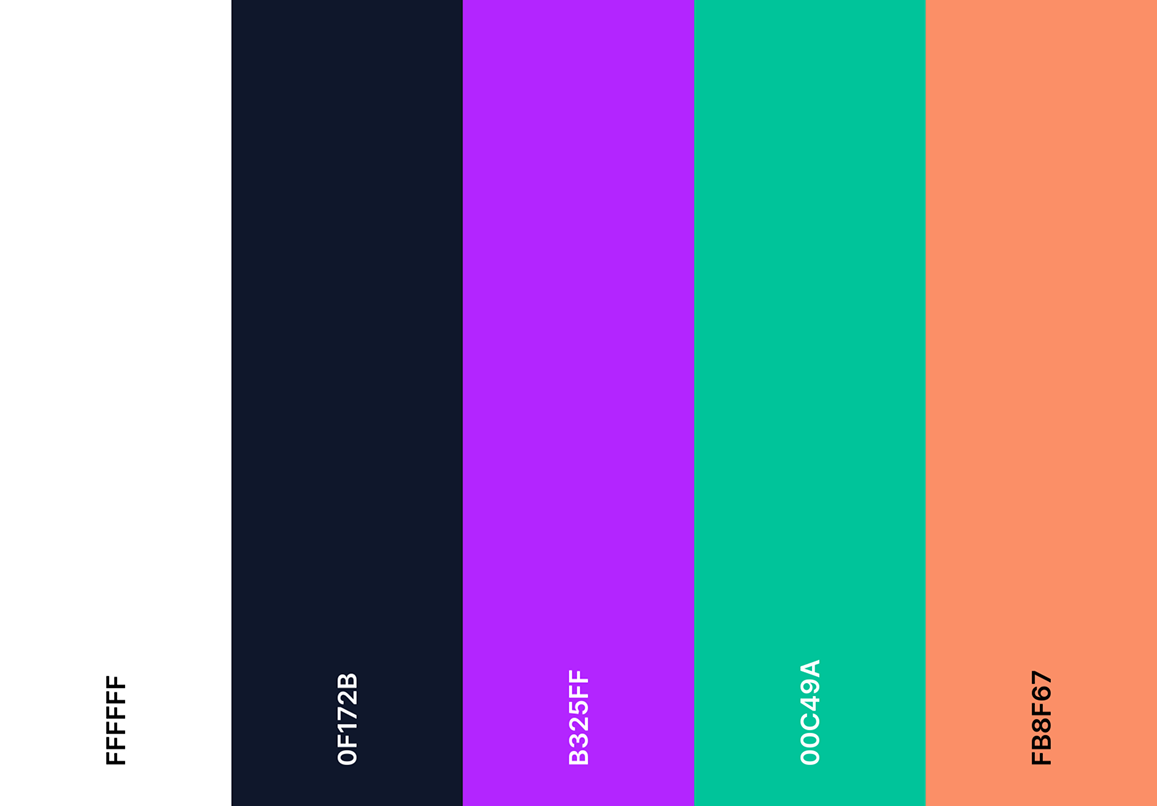
\includegraphics[width=\textwidth]{images/Colors}
        \caption{Color Palette}
    \end{minipage}
    \hfill
    \begin{minipage}[t]{0.48\textwidth}
        \centering
        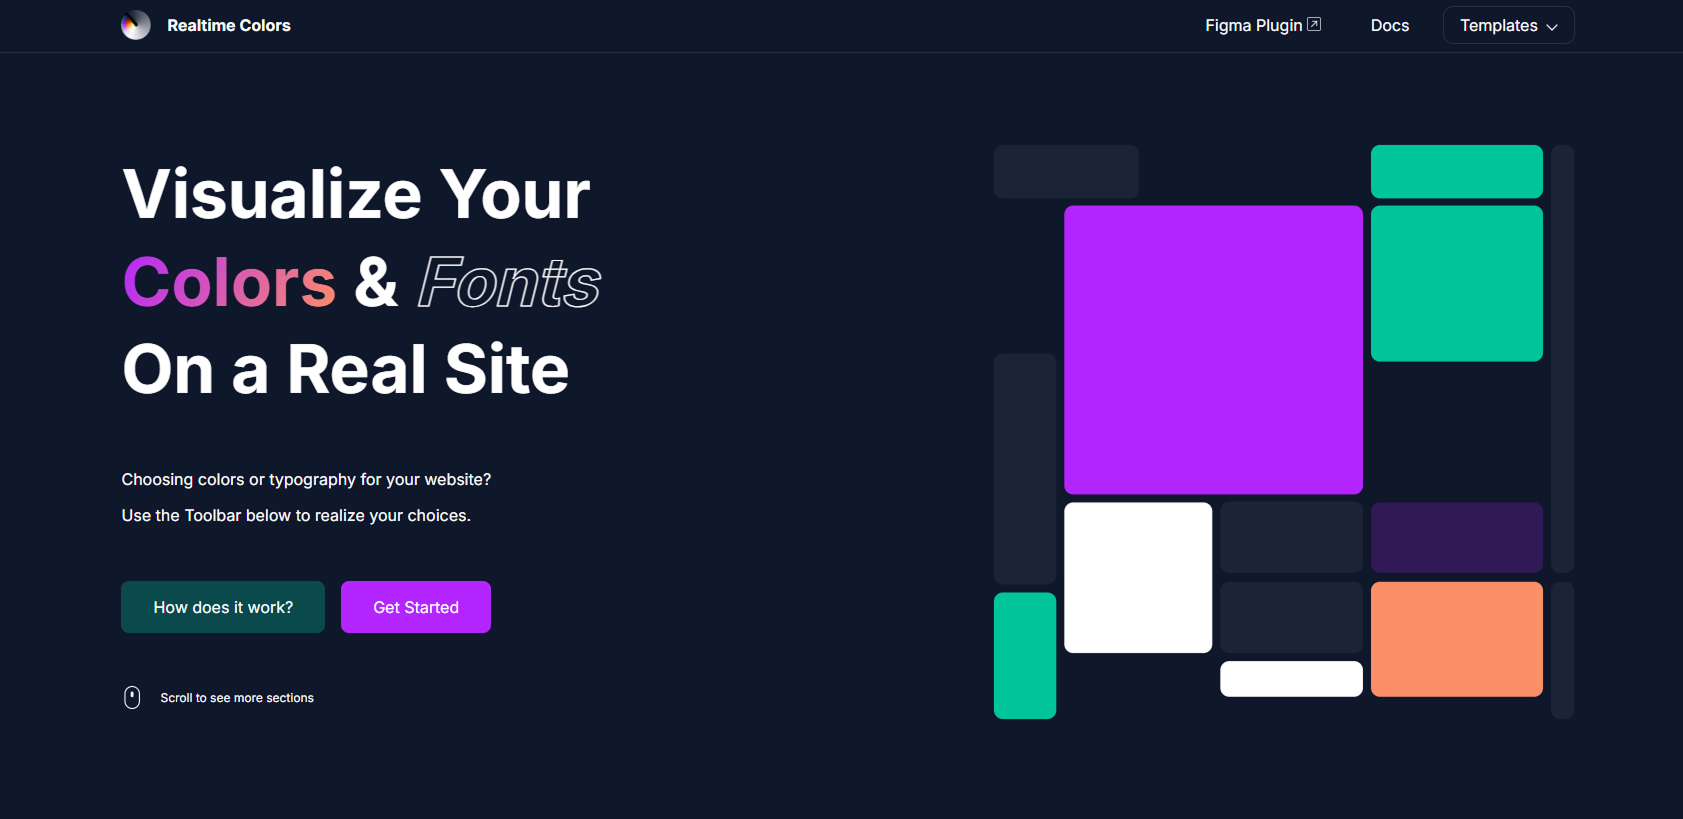
\includegraphics[width=\textwidth]{images/ColorsTested}
        \caption{Testing colors on mock website}
    \end{minipage}
\end{figure}

\subsection{Typography}

Use of a clean, sans serif font (Inter) with size variations for hierarchy and styling types (\textbf{bold}, \textit{italics}, etc.).
\\
\\
Clear typography improves legibility, especially when displaying tables, graphs, and dense statistics. Hierarchical font sizing (e.g., larger titles, medium subheaders, and small data text) guides the user's attention and helps separate elements visually without relying solely on color.

\begin{figure}[ht]
    \centering
    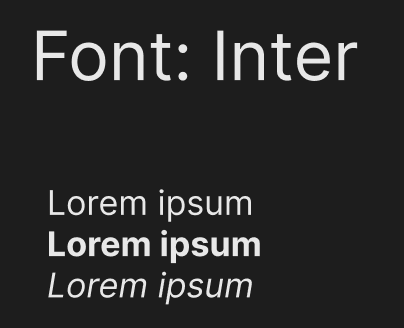
\includegraphics[width=0.3\textwidth]{images/Font}
    \caption{Font of the project}
\end{figure}